\documentclass{article}
\usepackage[utf8]{inputenc}
\usepackage{caption}
\usepackage{amsmath}
\usepackage{amssymb}
\usepackage{mathtools}
\usepackage{multicol}
\usepackage{graphicx}
\usepackage{wrapfig}
\usepackage{float}
\usepackage[makeroom]{cancel}
\usepackage{mhchem}
\usepackage{pst-plot}

\graphicspath{ {../images/} }

\renewcommand{\familydefault}{\sfdefault}
\renewcommand{\baselinestretch}{1.5} % line spacing
\newcommand{\fline}{\par\noindent\rule{\textwidth}{0.1pt}} % horizontal line (wide)

\title{Topic 9\\Lesson 1 - Oxidation + Reduction}
\author{Peter Zhang}

\begin{document}

\maketitle
\tableofcontents
\newpage

% lesson 
\section{Oxidation + Reduction}
Occurs in chemical changes whenever there is a shfit in \ce{e-} density from 1 atom to another.

\subsection{Oxidation}
The loss of electrons \ce{e-}

\subsection{Reduction}
The gain of electrons \ce{e-}

\subsection{Redox Reaction}
hen the oxidation and reduction occur at the same time. In the Bronsted-Lowry explanation of an acid, there will always be a base and an acid even if they don't show acidic properties.\\

\textbf{LEO the lion says GER}

\begin{itemize}
\item less electron oxidation
\item gain electron reduction
\end{itemize}

\pagebreak
\subsection{Rules}
\begin{enumerate}
\item use oxidation \# for all atoms in a reaction.
\item Any metals by themselves (natural/free) element form have an oxidation state of \textbf{zero}
\item In simple ions the oxidation state = change in \ce{e-}\\$$Ca^{2+} = +2, P^{3-} = -3$$
\item Oxidation states of all atoms in a netural compound must add up to zero\\$$\ce{MgSO3} = Mg (+2) + SO_{3}(-2) = 0$$\\Oxygen has oxidation state (-2) and Sulfur has oxidation state (4) \textbf{since Mg = 2 and O = -6} then S must be 2 to become 0
\item  \textbf{IMPORTANT} MAKE SURE THAT OXIDATION STATE IS (charge)(\#)
\end{enumerate}

\section{Polyatomic Atoms}
Oxiation state of polyatomic ions must add up to the charge of the ion $$NO_{3}^{-}$$We can now find the value of the oxidation state for each element. O = -6 (-2 * 3), overall = -1, therefore N = (-1 - (-6)) = 5.

$$\ce{N2 + 3H2 \rightleftharpoons 2NH3}$$

\pagebreak
\subsection{Redox Reactions Rules}
\begin{enumerate}
\item Start with half the equation - After identifying + separating what is undergoing oxidation + reduction
\item For each equation separately\\Balance the atoms \textbf{EXCEPT} H and O.\\Balance O by adding \ce{H2O} to opposite side.
\item Balance H by adding \ce{H+} ions\\This creates acidic redox reactions - \textbf{acidic redox reactions} (MAIN FOCUS OF IB -- but basic can also exist)\\ \textbf{If basic}: we add equal \# of \ce{OH-} as \ce{H+} to both sides of the reaction. The \ce{H+} thing still needs to take place even if it is a basic reaction. 
\item Balance each $\frac{1}{2}$ equation for charge. \\Add \ce{e-} to the side with more positive charge. \\\textbf{Normally} \ce{e-} added on product side = \underline{oxidation}\\\ce{e-} added on reactant side = \underline{reduction}
\item Double check all balanced so far
\item Equalize the \# of \ce{e-} to the 2 half equations by finding a common multiple. (\textbf{ELECTRON NUMBERS MUST BE EQUAL IN THE ENED}
\item Add the 2 half equations together and cancel out anything that is same on both sides.
\end{enumerate}

\subsection{Example}
\begin{figure}[H]
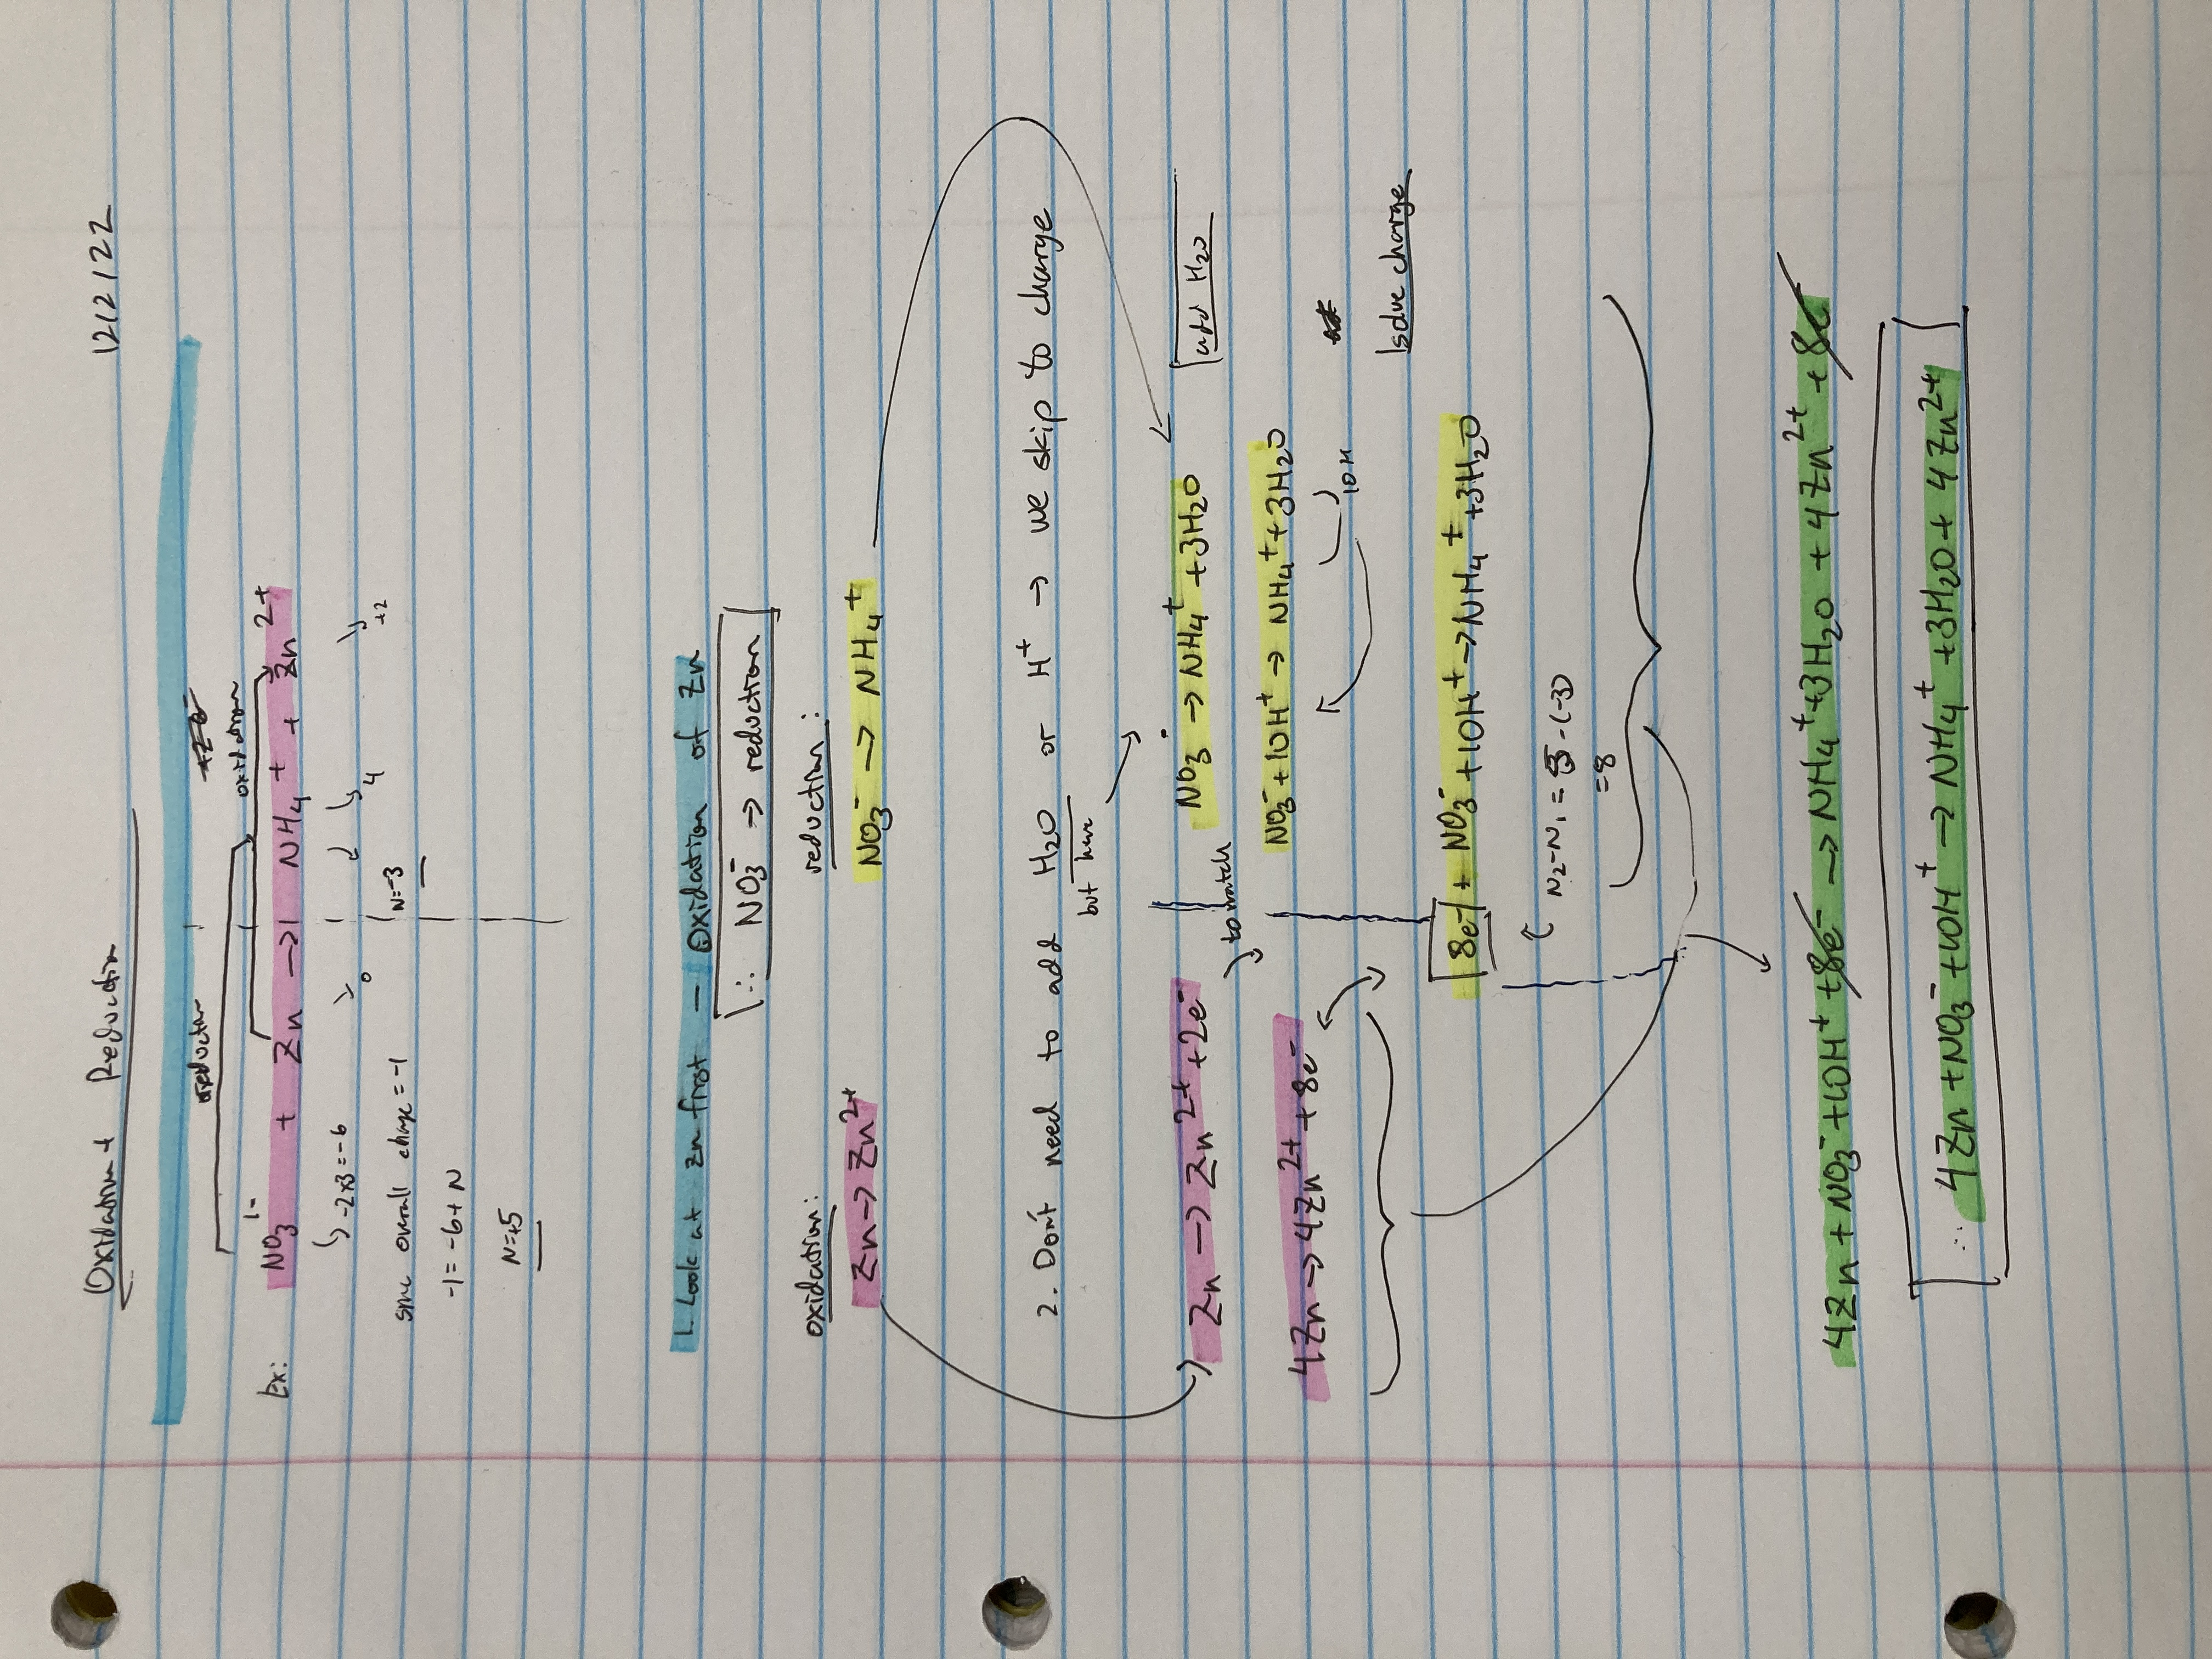
\includegraphics[width=\textwidth]{5.1fig1.jpg}
\captionof{figure}{How to solve Oxidation and Reduction Reaction}
\end{figure}









\end{document}